\documentclass[12pt,twoside,a4paper]{article}
\usepackage{titlesec}
\usepackage{chngcntr}
\usepackage{float}
\counterwithin{figure}{section}
\counterwithin{figure}{subsection}
\usepackage[margin=25mm]{geometry}
\linespread{1}
\titleformat*{\section}{\fontsize{14pt}{2}\bfseries}
\titleformat*{\subsection}{\fontsize{13pt}{2}\bfseries}
\titleformat*{\subsubsection}{\fontsize{13pt}{2}\bfseries}
\usepackage[T1]{fontenc}
\usepackage{listings}
\usepackage{mathptmx}
\usepackage{graphicx}
\usepackage{enumitem}
\graphicspath{ {imgs/} }

\begin{document}

Streszczenie:\\
Zakresem poniższej pracy jest proces projektowania i tworzenia urządzenia, które automatycznie przypisuje rozbite jajka kurze do jednej z dwóch poniższych klas:\\
\begin{enumerate}
\item nieuszkodzone żółtka otoczone białkiem jajecznym albo czysta linia produkcyjna
\item uszkodzone żółtka albo nieuszkodzone żółtka otoczone szczątkami uszkodzonych żółtek
\end{enumerate}
Implementacja urządzenia została poprzedzona badaniami, które porównują rózne metody oceniania obrazu z kamery, biorąc pod uwagę ich skuteczność pod względem zużycia zasobów obliczeniowych, oraz skuteczność klasyfikacji.\\
Działający prototyp został opracowany i jest w trakcie testów.\\
Urządzenie będzie masowo produkowane jako moduł wykorzystywanych w maszynie RZ-1 firmy OVO-Tech.\\
Zwiększy on atrakcyjnośc maszyny dla następujących grup odbiorców:\\

\begin{enumerate}
\item Firmy framaceutyczne, które produkują lekarstwa z białka jajecznego i stawiają wygórowane wymagania pod względem czystości białka jajecznego
\item Cukiernie, które wymagają czystego białka jajecznego do procesów piekarniczych takich jak ubijanie piany jajecznej.
\item Firmy produkujące odżywki dla sportowców
\end{enumerate}

Summary:
The scope of this work is process of creating a device that automatically assigns broken eggs into one of two following classes:
\begin{enumerate}
\item intact yolks surrounded with egg white or clear processing plant line
\item damaged yolk or intack yolk surrounded with damaged yolk parts
\end{enumerate}
The implementation of such device is preceded with research that compares various methods of recognizing the camera image, taking into account their performance in terms of computation resources, and in terms of correctness of the recognition.\\
The working prototype is sucessufully developed and tested.\\
The device will be mass produced as a module of OVO-TECH rz-1 egg braking machine, to improve machine usefullnes for following recipients:
\begin{enumerate}
\item Pharmacery companies that manufacture medicines out of egg-white and requrie high standards in terms of egg-white cleaness
\item Confectionaries that require clean egg white for baking procedures, such us egg foaming process
\item Athletes nutrition produers
\end{enumerate}



\tableofcontents



\section{Introduction}
\subsection{Research scope}
In 2014 creation of  camera based  module for chicken egg processing machines was requested by OVO-TECH company (the client).\\
The module is supposed to increase quality of egg-mass based  products made with use of  client machines.\\

During last 4 years multiple attempts were made by client to separate whites from yolks of freshly broken eggs in a mechanic way.\\ 
Obtained solutions proved to be working good enough for some companies, while other rejected them as imperfect and declared will to buy clients devices in the future, provided that adequate improvements will be made.

The scope of this thesis is overviewing the possibilities of resolving client needs with image processing mechanisms that will optically detect state of object (batch of  intermediate product) and judge whether or not it should be discarded from the processing plant.\\
Moreover, a process of creating a prototype device using tested method  is described.

Problems such as:
- choosing image preprocessing methods
- finding optimal  parameters for used image alternations
- overfitting issues
- real-device solution implementation, 
- technical issues concerning the device choice, setup and performance 
had been taken  into account during the research procedure.






\begin{figure}[H]
\centering
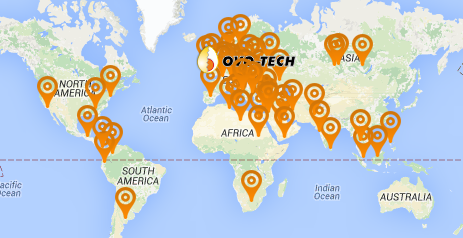
\includegraphics[width=0.4\paperwidth]{map}
\caption{Clients egg braking machines operating over the world}
\end{figure}

Figure 1.1 Clients egg braking machines operating over the world


\subsection{Host machine}
The machine that will be extended with the module prototype prepared in this thesis is OVO-TECH RZ-1 model.

\begin{figure}[H]
\centering
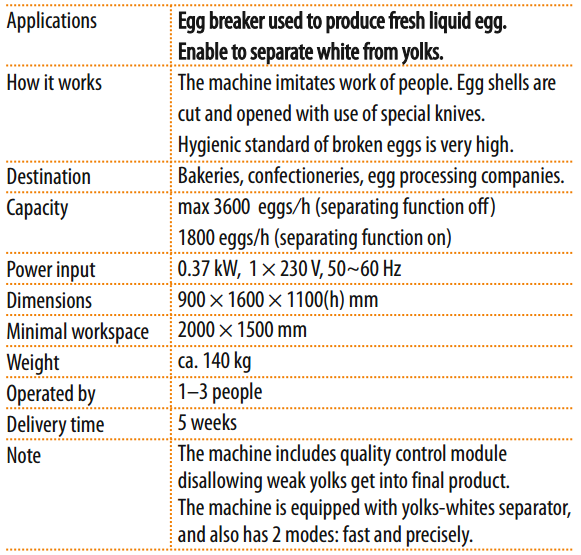
\includegraphics[width=0.4\paperwidth]{rz1table}
\caption{Rz-1 unit baisic parameters}
\end{figure}


\begin{figure}[H]
\centering
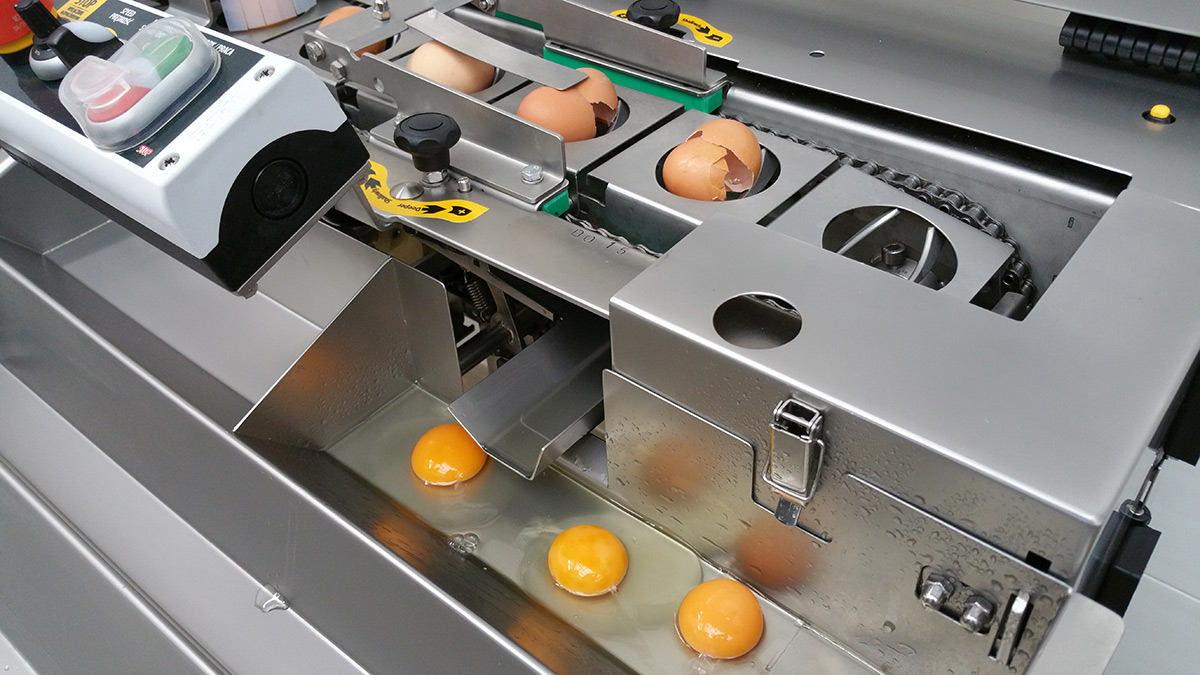
\includegraphics[width=0.4\paperwidth]{rz1crack}
\caption{Egg cracking  module of RZ-1 unit}
\end{figure}


The machine operates in a following way:
\begin{enumerate}
\item Eggs are directed into one-line flow, and mechanically aligned

\item Cracking module cuts the incoming egg surface from below with two knives that are aligned in direction of egg focal radius
\item The knives imitate human hands work by opening the previously notched egg
\item The cracked eggs are accumulated in a movable utensil for optical assessment. 
If the egg yolk appears to be broken, it is removed by an operator from the processing plant
\item Cracked eggs are transported by sliding to white and yolk separating module
\item Separation  is done in a mechanic way while eggs slide over specificly shaped gap that only egg white fills in, while the egg yolks remain intact
\end{enumerate}

\begin{figure}[H]
\centering
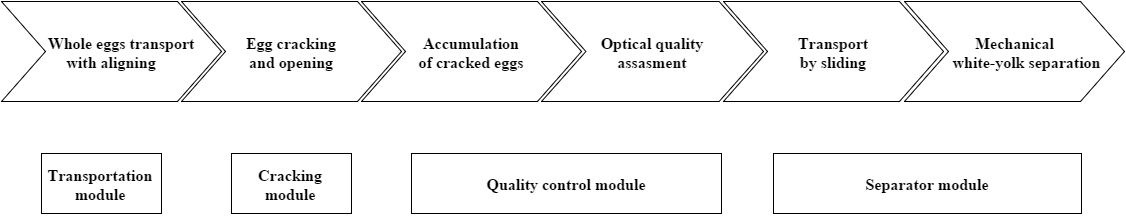
\includegraphics[width=0.8\paperwidth]{process}
\caption{RZ-1 Egg processing  - process and plant structure}

\end{figure}

RZ-1 operates in two modes:
- Precision mode
- Fast mode

Precision mode is used widely with bad quality eggs to extend amount of time for optical assessment in (5) phase.

More advanced OVO-TECH models such us RZ-3, RZ-6 and RZ-8 will be also considered for further research.

\subsection{Problem description}

If an egg processed by rz-1 machine is old or the chicken was feed improperly the yolk might be either broken already inside the egg, or might break during the cracking  phase due to cracker imperfections such us being calibrated for different size or weight eggs.\\
A mixture of damaged yolk and white is created in a result, and it’s not possible to separate it into two initial components using  the rz-1 separation  module.

Batch of such mixture should be removed from  the processing plant, since it would contaminate pure egg white product otherwise. 

\begin{figure}[H]
\centering
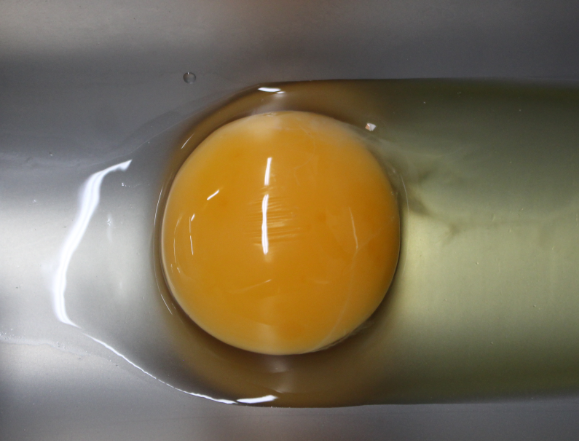
\includegraphics[width=0.4\paperwidth]{prop}
\caption{Properly cracked egg}
\end{figure} 

 
\begin{figure}[H]
\centering
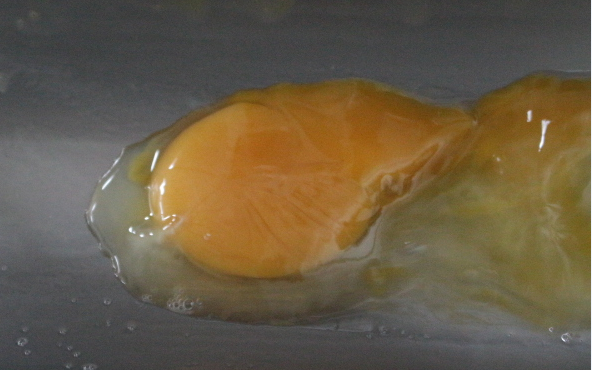
\includegraphics[width=0.4\paperwidth]{damg}
\caption{Damaged yolk in improperly cracked egg}
\end{figure}

\subsection{Demand for improvements}

Nine companies were inquired whether or not would they invest in improved Ovo-tech machine, provided that egg white will be visually clean of yolk parts.\\
Seven of them replied positively that they would seriously consider such offer since their processing plants would benefit in terms of product quality or manpower cost on such improvement.\\
Remaining 2 companies did not answer the question.

One should consider why better separation is a requirement for those companies.\\
Following reasons were presented:

- Confectionaries and bakeries utilize egg white foam as an ingredient for their products.\\
Egg white foam is obtained by aeration (also known as beating / foaming / whipping) process.\\
Comprehensive process description was provided by one of the bakers:

"When air is incorporated into a liquid or viscous solution, the solution entraps the air bubbles, forming a foam. If the foam is stabilized by proteins, it leavens a food, increasing its height and reducing its density. The viscosity of all egg products is ideal for incorporating air cells during the whipping or beating process. As whipping or beating progresses, air bubbles decrease in size and increase in number, all the time surrounded by egg proteins. Liquid egg products have low air-liquid interfacial tension; thus, when eggs are beaten or whipped, the proteins denature, or simply, they unfold. This exposes two oppositely charged ends of the protein molecule: the hydrophobic, or water-hating end, and the hydrophilic, or water-loving ends. The proteins align themselves between the air and water, securing the air bubbles with their hydrophilic chains pointing into the water and dangling their hydrophobic chains in the air. During baking, these proteins bond with each other, forming a delicate, yet reinforced network.

Egg whites do this much better than yolks because of the unique proteins found in whites. In fact, even though the term foam technically refers to any system where there are entrapped air bubbles, in the food industry, when discussing egg white products, the term tends to be exclusive to egg whites foams. This is because egg whites, unlike any other natural food ingredient, are able to create the largest possible food foam, a foam six to eight times greater in volume than unwhipped, non-aerated liquid egg white

Whole eggs and egg yolks can also increase the volume of foods, including certain baked goods and dairy desserts such as ice cream and custard, but just not as much as egg whites alone. Visually, whipped yolks may double or triple in volume, while whipped whole eggs produce less volume than either yolks or whites whipped separately. They are also less thick than yolks alone." \cite{eggprop}

- Ovo-tech observed that a simple dependence exists: the older the egg is, the more likely its yolk is degenerated inside the egg shell.
Thus eliminating the batches containing fuzzy yolk should decrease chances of accidentally processing the contaminated eggs, while the risk of egg contamination generally increases with egg age.

- One of the Ovo-tech clients is a biotechnology company that manufacture medicine out of genetically modified eggs.\\
The company purchased some ovo-tech machines, but is nevertheless displeased with their separation ratio.\\
This company currently is undergoing a procedure of obtaining US Food Drug Administration (FDA) approval for wide distribution of their egg-based medicine.\\
Executives of this client suspect that using machines with better egg separation will increase their chance for positive outcome of above process.\\
A non-disclosure agreement was signed between this client and ovo-tech, thus further expanding this topic in scope of this thesis is not possible.

\section{Problem analysis}
\subsection{Establishing framework for product cleanness assessment}

The requirement is to create a system able to detect all badly-cracked eggs.\\
After request for clarification, client made 60+ pictures of product during machine operation and classified them manually, thus requirement is less ambiguous.

Client decided that intact egg yolks should be removed from processing line if:

\begin{enumerate}
\item intact yolk is surrounded by homogeneous mixture of another damaged yolk and white.
This is the most strict (in terms of cleanness) case, that generates less strict cases:
\item intact yolk surrounded by damaged yolk blobs
\item fuzzy (damaged) yolk that still keeps its shape without mixing with white
\item damaged egg blobs surrounded with white
\item egg-white homogeneous mixture
\item egg-white nonhomogeneous mixture
\end{enumerate}
Two cases are accepted as proper product:
\begin{enumerate}[resume]
\item intact yolk surrounded with egg white
\item clean egg white
also, there is no need to do anything when:
\item transportation part is empty (machine is not operating or the operators are preparing next batch of eggs).
\end{enumerate}

 

\begin{figure}[H]
\centering
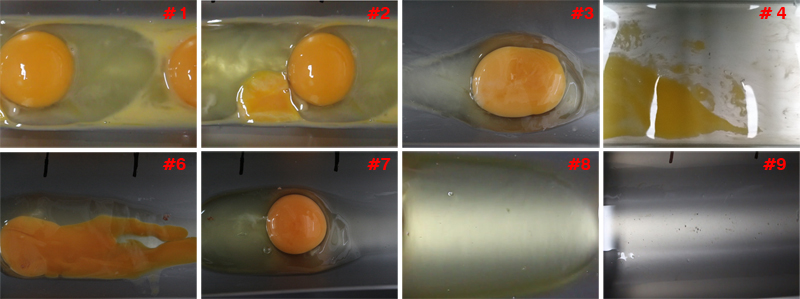
\includegraphics[width=0.8\paperwidth]{8of9}
\caption{Cracked egg product cases. Source: own materials }
\end{figure}
Source: own materials 

Also, a problem is constituted by chalaza - a usually white element that is attached to egg yolk for in-egg suspension.\\
Despite the fact, that client decided that chalaza position and amount are irrelevant to him, its appearance may increase difficulty of the recognition problem if identified as parts of damaged egg yolk.

 
\begin{figure}[H]
\centering
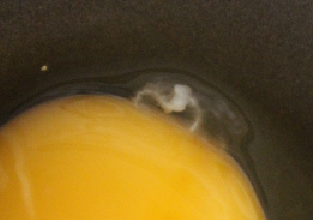
\includegraphics[width=0.4\paperwidth]{chalaza}
\caption{Chalaza attached to egg. Source: own materials}
\end{figure}


\subsection{Techniques of automatic egg quality assessment}

Different techniques for automatic, non-destructive egg quality grading have been investigated.
Among them, the following are worth mentioning:
\begin{itemize}
\item Intelligent systems based on visible-infrared transmittance spectroscopy\cite{agri}
\item Fourier frequency analysis of a vibration-based response on impact force\cite{svm} 
\item Ultrasonic, magnetic resonance, electric resistance, electric nose\cite{nondestr}  
\end{itemize}
All methods listed above require very specific equipment, are prone to overfitting and take in to account assumption that does not has to be satisfied for problem considered in this thesis: the egg shell should not be damaged.

Since in this very special case, eggs are already broken, simplified and different methods can be considered.
Initially, two ideas were researched by author of this thesis:
\begin{itemize}
\item Proximity sensor utilization
\item Using laser / narrow light beam 
\end{itemize}
Both methods would identify the intact yolk basing on its height and wouldn’t require much processing (an Arduino Uno or other ATMega based circuits might be sufficient).\\
Nevertheless, both of them had to be rejected, since intact yolks presence in the tested batch is not sufficient for batch accepting – absence of egg yolk parts is also required (see subchapter 2.1).\\
Finally, using images of the batch obtained from camera and processing it was chosen as a most promising option for further research.









\section{Batch state detection system design}

\subsection{System structure}
The system is expected to replace Quality control module (See. Figure 1.2.3).\\
The egg acumulation will not logner be required, as well as the work of qualified expert that opticaly assased the egg quality is not needed anymore.\\

A camera will be placed on top of Separator module part, where cracked eggs are transported by sliding to the separating part.\\

The processing device will use the frames of camera image. Some of the frames will be skipped to reduce amount of data.\\
Frameskipping ratio depends on decision algorithm and device performance.\\

The processing device will use the frames, to make a decision whether or nor the egg barch visible on the frame is acceptable, or represent a badly cracked egg.\\
A signal will be send to element that will either remove egg batch from the processing plant or let is pass further.\\

Development of this physical element is done by OVO-TECH company and is not analised in the thesis. OVO-TECH declared, that having +5V signal for positive batch, and -5V for negative is enough for them to work on their part.


\begin{figure}[H]
\centering
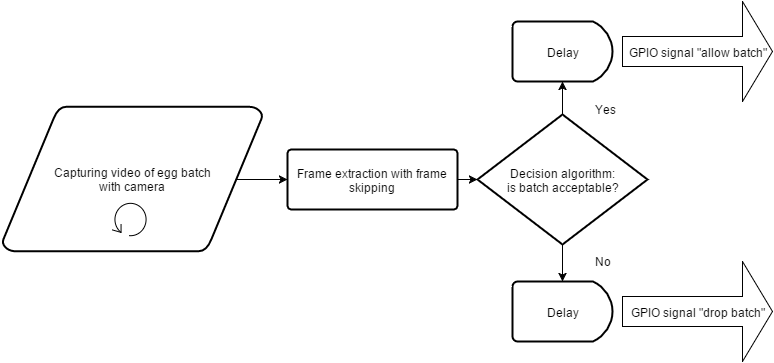
\includegraphics[width=0.8\paperwidth]{system}
\caption{System structure}
\end{figure}



\subsection{Detecting batch state with camera image}

When it comes to assessment of camera image, 4 approaches are widely considered:
\begin{enumerate}
\item Very easy scanning with photo sensors or very low resolution cameras
\item Computer graphics preprocessing and segmentation accompanied with assessment of a parameter (number of pixels, number of feature points, percentage of one region that fills another bigger region and similar)
\item Machine learning approach
\item Neural networks which are used as a special case of either machine learning process or a part of it 
\end{enumerate}
First case was considered, since it could be implemented on Arduino Uno, other ATMega based platform or real-time systems working on PLC controllers such as LOGO! 7, which are often used in factories due to their reliability (apart from Stuxnet-class worms, that has been firstly observed in 2010, no other security threads are believed to exist).\\
Unfortunately, the problem is more complex than simply deciding whether the product is present or not; or whether the product is yellow or not, thus more advanced processing is required.\\

Second case will be expanded in the next subchapter and has been chosen as main method that will be implemented and tested in this thesis.\\

Last two approaches will be tested if the 2nd approach will provide to be insufficient.\\
It is worth mentioning, that for (3) Support Vector Machines was considered, since it classifies data to exactly two classes (i.e. proper and improper egg mass).\\

Also, Haar Features Cascade was tested, but data amount obtained for testing was insufficient, and the methods popular implementations are focused on locating the particular object on image rather than on comparing two pattern cases.\\

(4) Case was considered and the author build a multilayered perceptron network working with MNIST database in order to better understand the method.\\
The method application will be researched further on beyond the scope of this work.



\subsection{Detection algorithm}

Frames are acquired from the camera module.

Than, two copies of the frame are processed independently.

\begin{description}
  \item[Firstly,]one channel is extracted from the image.\\
  Its state is passed further as image, along all the steps.
  \item[Secondly,]the channel is a subject to preprocessing, that eliminates the unimportat data and reduces the data dimentionality.\\ 
  Amount of noise is reducted.
  \item[Thirdly,]the image is segmentated, and the shape recognition methods are used to detect existance, position and size of the egg yolk.
  \item[Independently,]other copy of the image is a subject to different color scale.
  \item[Then,]only one channel is extracted from the image
  \item[Finally,]the information from first copy is used to remove intact egg region from second copy.\\The first copy is no logner needed and its rresources are freed.
\end{description}

Choosen channel of transformed second copy (with intact egg excluded) serve as the only image now.\\
It is processed in a following way:

\begin{description}
  \item[Firstly,]an attempt is made to dilter out the light reflections and flares from the image.\\
  Hopefully, during the further development, above artifacts can be removed in a phisical way, by mounting and lighting the device in a very specific way.\\
  For now nevertheless, this step is necessary.\\
  \item[Secondly,]image is segmentated with thresholding.
  \item[Thirdly,]noise (defined as small blobs) is deleted.
  \item[Finally,]the obtained image is expected to contain only unwanted, damaged egg mass.\\
  Amount of pixels contaning it is counted.
  \item[Decision] is made basing on the obtained amount.\\
  It takes a form of signal sent to phisical element that either removes the egg batch or let it through.
\end{description}

The best obtained combination of preprocessing, segmentation and grading parameters will be used in a final algorithm that will be implemented in Raspberry Pi 2 device with camera module, and than tested in the Rz-1 processing plant.


\begin{figure}[H]
\centering
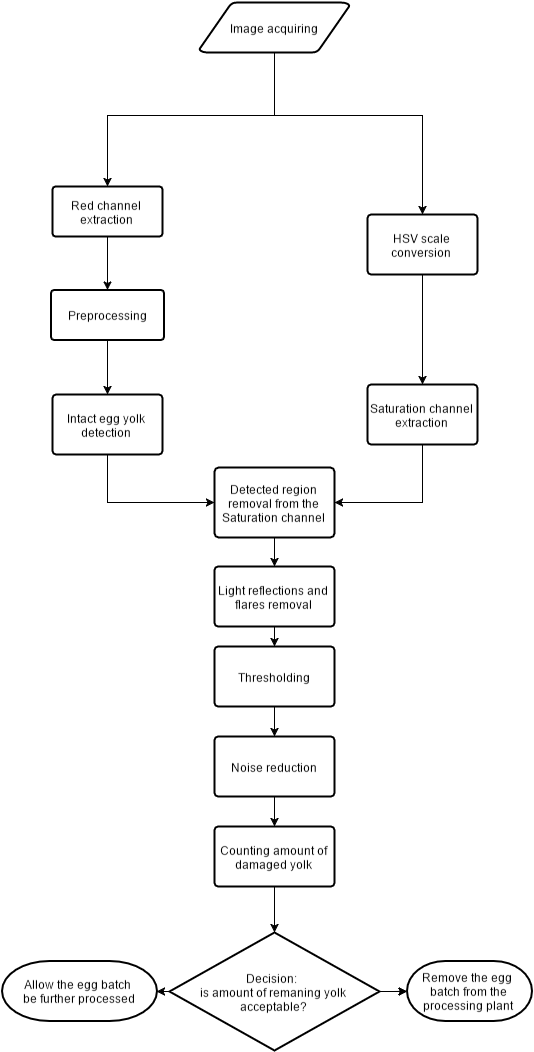
\includegraphics[width=0.5\paperwidth]{algorithmV}
\caption{Detection Algorithm}
\end{figure}


\subsection{Algorithm programming}
Decision have been made, to utilise OpenCV computer vision library for batch state recognition.\\
OepnCV is designed for computational efficiency, with strong focus on real-time applications.\\
It has been written in optimised C and takes advantages of multicore processors.\\
It provides simple-to-use interfece that enables building sophisticated computer vision solutions.\\
The library features more than 500 functions that process images, a general Machine Leraning Library (including Multilayered Perceptron Networks).\\
It is used since 1999 by major institutions such as Stanford University and is mantained and developed by specialists from companies such us IBM, Microsoft, Intel, Sony, Siemens, and Google.\cite{learnopencv}

First recognition attempts were done by the author of thesis using Android 4.3 running on Samsung N7100 Galaxy Note II smarpthon, utilising its build in camera.\\
The initial code was written with use of Java distribution of OpenCV library, as well as Android SDK.\\
Sadly, the performance of developed pre-prototype was very poor and a single frame was processed in more than 3 seconds.\\
Another version was build in a way that most resource consuming operations (such us Hough Circle Transform and all array operations) were rewritten in C language.\\
For that purpouse original C version of OpenCV was utilised, as well as NDK (Native Development Kit for Android).

Nevertheless, author of this thesis, decided that despite Android aviability for embedded platforms, it is no a platform suitable for factory tasks, due to big overhead, long booting and variety of functions that will not be utilised.

Raspbian Linux "Jessie" distribution was picked as the adequate one to host recognition algorithm accopmanied with Python 2.7 language.\\
Python is well supported on Raspian, it produces small amount of code, and can be executed fast in terms of computational time if the speciffic C-written functions are called.\cite{performance}\\
For author, a case occured, that 39-lines code snippet that recognise nested regions of image, written in C took only 6 code lines after rewritting it in Python.


\section{Egg yolk detection}
\subsection{Methods overview}
An egg yolk, when intact and fresh can be approximated with sphere which projects as circle-like shape on 2D image.\\
Methods presented below enable to filter out the unnecessary noise, simplify the image and detect the yolk shape.\\
While not all of them were used in the final detection algorithm, they were giving promising results on the early stage prototypes.

Following methods treat images as 1, 8, or 24-bit encoded matrices, thus both terms are used synonymously.\\
x and y denote pixel position.

\subsection{Circle Hough Transform (CHT)}
Circle Hough Transform is an algorithm used for retrieving 3 parameters defining a circle-like shape on images\cite{hgtcv} : 
- (xc, yc) - position of shapes center
- r - its radius

To understand the way CHT works, simplified case is considered:\\
The image is 1-bit encoded; the radius r and position (xp,yp) of a point lying on the searched circle are known.\\
Potential circles space is created by treating points on a circle of radius r centered in (xp,yp) as centers for potential circles.\\
For every potential circle, number of intersecting points is counted.\\
The potential circle with largest number of intersections is chosen as the best fitting one.

 
\begin{figure}[H]
\centering
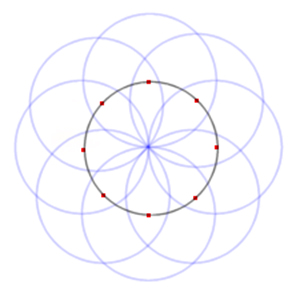
\includegraphics[width=0.4\paperwidth]{space}
\caption{Potential circles space\cite{craters}}
\end{figure}

In the full cases, such procedure is repeated for every image point, and the intersections numbers are stored in accumulation matrix.\cite{hgt}\\
To reduce computation time and false detection rate, minimum distance between image centers is given as a parameter min-dist.\\
Threshold value param-2 is defined as minimum number of intersections to treat circle candidate as detected circle.
 
\begin{figure}[H]
\centering
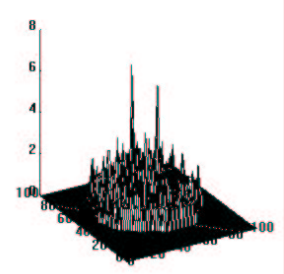
\includegraphics[width=0.4\paperwidth]{accu}
\caption{Accumulation matrix with two good circle candidates\cite{hgt}}
\end{figure}

If r is unknown, min-radius and max-radius parameters are defined, and the algorithm repeats the procedure for all possible integer r in range of above parameters.\\
OpenCV utilizes Canny edge detector for finding the potential intersection points, thus operates not only on 1-bit images, but also in 8-bit grayscale and 24-bit bgr images and provides smaller number of false positives.\cite{mastercv}\\
param-1 is introduced as higher threshold for Canny edge detector, while the lower threshold is set to 0.5 * param-1\cite{fd} .


\subsection{Erosion and Dilatation}
Erosion and dilatation are two morphological filters that enable to filter out unnecessary noise from the image.\\
Combined, they leave the core information (biggest blobs) intact or amplified, while small elements are deleted.\\
It is easily applied to binary images:\\
A ROI (region of interest, a rectangular part of image) moves through image pixel by pixel and is compared to previously defined kernel (binary matrix, usually symmetric with respect to both diagonals).

 
\begin{figure}[H]
\centering
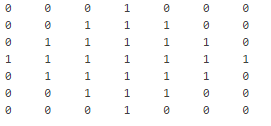
\includegraphics[width=0.4\paperwidth]{diam}
\caption{A diamond-shaped kernel\cite{morph}}
\end{figure}

The consecutive pixels of on ROI that matches kernel elements with value 0 remain intact.\\
Pixels of ROI that matches kernel 1-valued elements changes to:\\
1-ns if at least one of them is 1 for Dilatation\\
0-s if at least one of them is 0 for Erosion.

Erosion gives the effect of ‘shrinking’ the objects (and if they are small enough, they are deleted).\\
Dilatation makes the objects bigger.

 
\begin{figure}[H]
\centering

\includegraphics[width=0.4\paperwidth]{lett}
\caption{Orignal image, eroded image, dilated image.\cite{erdil}}
\end{figure}


When these methods are used multiple times, and convoluted, they filter out the noise.\\
Perimeter Determination and Skeletonization are widely used contour detection functions which utilize erosion and dilatation\cite{erdil}.


\subsection{Gaussian blur}

Gaussian blur is obtained by convoluting pixel with gauss function values. 

It reduces noise, detail and filters out the high frequencies what makes it a low pass filter.\cite{cv}

Gaussian blur drastically reduces number of false-positive Hough circles detections. It nevertheless should be coupled with sharpening to reduce false-negative cases.\cite{cnoisy} 


\begin{figure}[H]
\centering
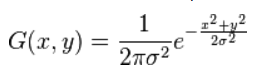
\includegraphics[width=0.4\paperwidth]{gauss}
\caption{Gauss function in two dimension\cite{featproc}}
\end{figure}


sigma, ksize.width, ksize.height  parameters are introducted.\\
Ksize stands for size of precomputed kernel, that is convoluted with ROIs on the image.

The term ‘convolution’ might be misleading and for the scope of image processing tasks is defined as picewise multipling two matrices and than summing the obtained values:

 
\begin{figure}[H]
\centering
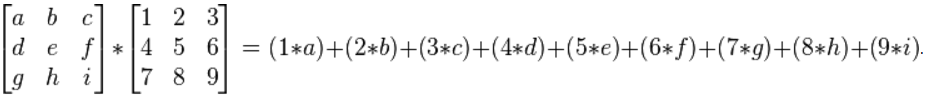
\includegraphics[width=0.8\paperwidth]{conv}
\caption{Convolution of 3x3 matrices\cite{gimp}}
\end{figure}

 
\begin{figure}[H]
\centering
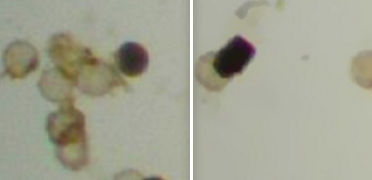
\includegraphics[width=0.4\paperwidth]{micro}
\caption{Microscope image before and after applying gaussian filter\cite{cnoisy}}
\end{figure}

  


\subsection{Channeling and HSV conversion}
lorem ipsum
\subsection{Using the methods}
\lstinputlisting[language=Python]{yolk.py}

\section{Contaminated product recognition}
\subsection{General idea}
lorem ipsum
\subsection{Thresholding}

Thresholding is a simple case of image segmentation.\\
It can be used to convert one channel (in most cases grayscale) image to binary image.\\
The basic binary thresholding mode sets every pixel of destination matrix to:
\begin{itemize}
\item 0 if the source matrix value is smaller than threshold (integer parameter)
\item 1 if the source matrix value is bigger than threshold.
\end{itemize}
The truncate version sets every pixel of destination matrix to
\begin{itemize}
\item threshold if the source matrix value is smaller than threshold, or
\item leaves it unaltered otherwise.
\end{itemize}
Various modes and modifications are used depending on coding schema and colors distribution.
  
\begin{figure}[H]
\centering
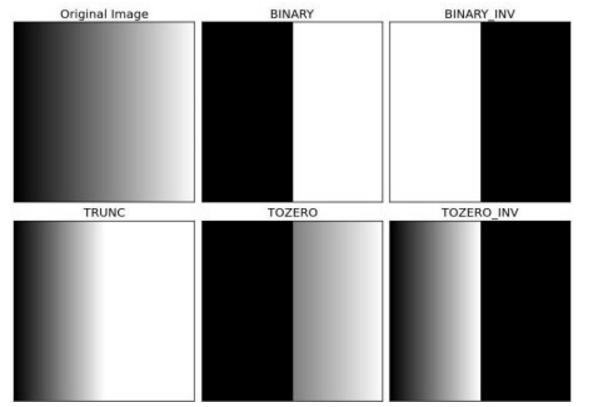
\includegraphics[width=0.4\paperwidth]{thr}
\caption{Different Thresholding modes generated with Metaplotlib}
\end{figure}



Finding optimal threshold value finding is a time consuming process and it often gives satisfactory results only for small set of images.\\
Therefore Otsu Binarization algorithm for automatically selecting threshold is used.

Moreover using one threshold value for whole image may not work properly if the lighting conditions differ in different image areas.\cite{thre}\\
Adaptive Thresholding utilize different threshold values for different ROIs.\\
Two modes are often used: Adaptive Mean and Adaptive Gaussian.\\
First compute threshold value as mean of neighborhood values.\\
Second uses weighted sum neighborhood values.
 
\begin{figure}[H]
\centering
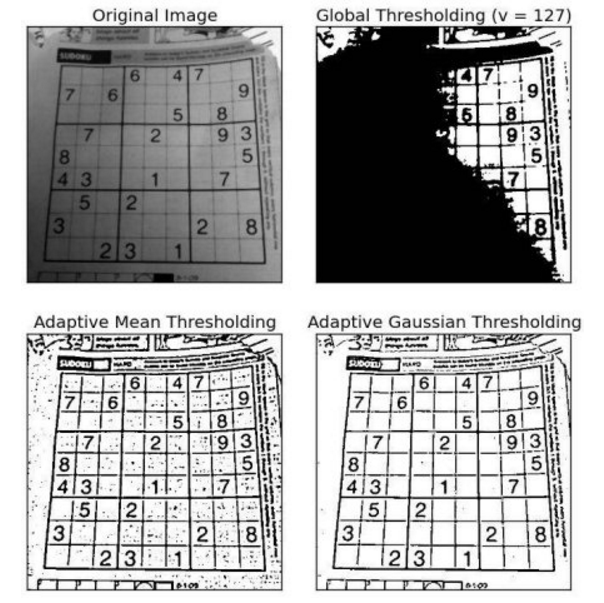
\includegraphics[width=0.4\paperwidth]{thremeth}
\caption{Threshold computing methods12\cite{thre}}
\end{figure}
 
\begin{figure}[H]
\centering
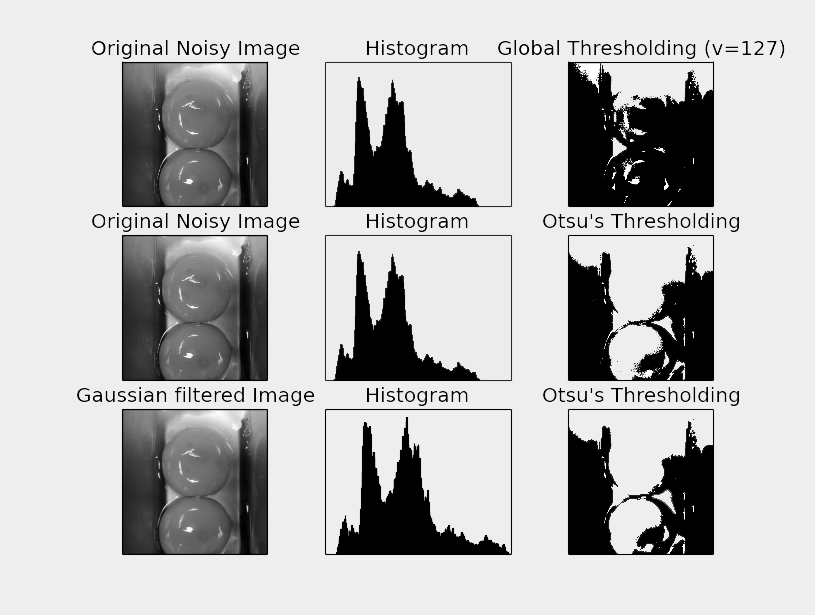
\includegraphics[width=0.4\paperwidth]{diffthr}
\caption{Different thresholding applied
Fig. generated with Metaplotlib}
\end{figure}


For more general cases (i.e. multichannel images, assigning more colors) clustering method known as k-means is widely used.\cite{lesscv}
 
\begin{figure}[H]
\centering
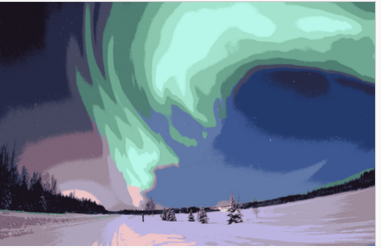
\includegraphics[width=0.4\paperwidth]{kmeans}
\caption{K-means clustering method for k = 16\cite{segm}}
\end{figure}
\subsection{Using the methods}
\lstinputlisting[language=Python]{contaminated.py}

\section{Choosing detection system parameters}
\subsection{Manual parameters finding}

There exist a set of parameters that define the mode, that previously explained methods operate as well as their instensivity.\\
Finding optimal values of this parameters is a hard task, since for example CHT method didn't found a single egg yolk with defualt numbers.\\
The following values have to be found:
\begin{description}
\item[param1] - lorem ipsum
\item[threshold] - lorem ipsum
\end{description}

A script was developed, that displayed over 500 pictures for 0.3 second each in a loop.\\
Trackbars was displayed above the frames, with every trackbar coresponding to one parameter that is supposed to be chosen.\\
Beside, the already transformed frames after transormations were shown.\\
The expert was reviewing the output while changing the trackbar positions to obtain an image that segmentates the egg yolk properly.\\



\begin{figure}[H]
\centering
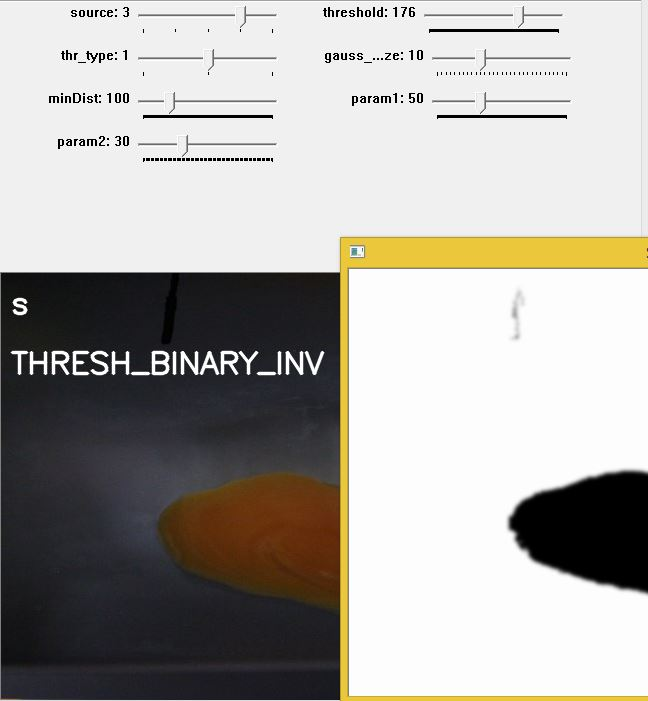
\includegraphics[width=0.5\paperwidth]{manual}
\caption{Screen of running one of the scripts used for manual parameter finding}
\end{figure}

Script crucial fragments:

\lstinputlisting[language=Python]{trackbars.py}

Unfortunately, while some parameters sets worked fine for some image sets, they failed with another ones.\\
Nevertheless, the interesting intervals were obtained for each trakcbar. These intervals guaranteed that at least some of the graded images are segmentated in exptected way.\\
This method resulted in excluding most parameters values and vastly reducting the optimising problem size.

\subsection{Automatic parameters finding}

A decision was made, to automatise process of assesing the segmentation and detection efficiency to get to optimal set of parameters.\\
This process was done twice:\\
\begin{description}
\item[Firstly,] the egg yolk detection process was optimised.
\item[Secondly,] the contaminated product detection utilising the previously otpimised egg yolk detector was perfected.
\end{description}

To accomplish first objective, avaliable images were devided into 3 subsets for first process:\\
\begin{itemize}
\item 0 intact yolks visible in a frame
\item 1 egg present
\item 2 eggs present
\end{itemize}
For the whole set, the recognition error was defined  as sum of missdetections for every subset.\\
A simmilar procedure was conducted for second objective: the same images were devided into following subsets:
\begin{itemize}
\item Contaminated batches
\item Batches with either only intact eggs or no egg mass at all
\end{itemize}
Error was defined as false negatives (good batch recognised as bad batch) number summed with false positives number multiplied by 3.\\
Multipilication by '3' weight was conducted on false positives, since keeping the product clean is more important for the client, that utilising all the egg mass. 

A script was developed, that automatically loaded the images and graded them for different parameter values.\\
This process was very expensive in terms of processing time, and the parameters range and step was choosen to fill a night of i7-3520M 8GB RAM computer work.\\
It was computed in a following way: elapsed time of one full imageset testing multiplied by number of possible paramter sets.\\
The process was repeted by the author multiple times with different parameter intervals discovered in a process descriped in previous subsection.\\
Various effort were made by the author to optimise imageset grading process, so bigger variety of parameters can be checked.\\
Initialy, files were open prior to every image evaluation, later on all the images were loaded once, and every processing (channel spliting, colorscale conversion) was conducted before execution of the code nested in multiple loops.

Crucial parts of the testing code:
\lstinputlisting[language=Python]{script.py}


\subsection{Overfitting}
Overfitting is an unwanted effect that appears often in statistics and supervised machine learning.\\
Overfitting means, that parameters of some model are fitting the specific modeled data case, rather than the general model.\\

In this case it means, that the parameters of image processing that were found, maximise the recognition efficiency for the data provided by OVO-TECH, while a new data (with different kind of eggs, different kind of noise or with images made in different conditions) can be classified in improper way.\\

Overfitting occurs mostly if:
\begin{itemize}
\item A set of sample data is too small
\item A set of sample data is not diverse enough
\item No regularisation or cross-validation methods are used
\end{itemize}

To reduce this effect, author used different dataset for getting the transform parameters, and different set (excluded 10% of data from every sample subset) for assesing the recognition quality.

During protoype in factory testing and further development this issue will be addressed in extended way.

\section{Phisical system implementation}
\subsection{Phisical Platform}
\subsection{Camera module}
\subsection{Programming raspberry pi}
\lstinputlisting[language=Python]{rpi.py}
\section{Further research and development}

Work on the solution developed in this thesis will be continued further on by the author and OVO-TECH company.\\
The following alternative approaches and improvements in detection system will be taken into consideration
\subsection{Operating Systems}
Using alternative system operating on Rasperry Pi 2 platform might improve image processing performance. Therefore, more frames per second could be analized, more filters can be applied and higher resolution pictures could be used.
Among over 20 avaliable ARM systems, presented below are most promising:
\begin{itemize}
  \item Minibian - a Raspbian image that is resource optimised.\\
  Its current Raspian "Jessie" based version boots in 14secs, use only 29MB RAM and takse 451MB (compared to 1,2GB in original version). \\GUI, aplication clients, office suite and other non-necessary packages have been removed.\\ The image is targeted for embedded or server applications (NAS, Web server, electronic applications).
  \item Arch Linux ARM
  \item Gentoo
  \item SliTaz
  \item Windows 10 IoT Core - embedded solution developed by Microsoft. Guarantees extensive technical support.
\end{itemize}

Largest reliability and performance benefits are expected from using realtime-capable systems.\\
Following solutions are avaliable or developed for Raspberry Pi:

\begin{itemize}
  \item RISC OS
  \item Xenomai
  \item PREEMPT\_RT kernel patch and High Resolution Timers\cite{stackos}
  \item ChibiOS/RT\cite{chibi}
  \item RODOS - an Open Source kernel project developed by the German Aerospace Center and Prof. Montenegro's University\cite{rodos}
\end{itemize}

Nevertheless advanced image processing, GPU access, utulisation of existing graphics libraries might be not avaliablie or require amount of effort unproportional to those benefits.\\
Also, external real-time clock (such as AD9850 Pulse generator) might be required.

\subsection{Platforms}
\begin{itemize}
  \item Arduino Uno R3 accompanied with DS1307 Real Time Clock - considered, but for now the image processing is to extensive in terms of image processing.\\
  Having extremly cheap clones (4-20\$ on retail market) that fetures often stronger ATMega units is an advantage altough.
  \item Intel Galileo Gen 2 - based on Intel Quark 32-bit SoC X1000 processor, provides pins-compatible with shields designed for the Arduino Uno R3, what makes communication with other OVO-TECH machine modules easier and allows use of the mentioned above RTC.
  \item PandaBoard - the OMAP4430 features 1 GHz dual-core ARM Cortex-A9 MPCore CPU (a big improvement compared to Cortex-A7 CPU in Raspberry Pi 2), 304 MHz GPU, and 1 GiB DDR2 SDRAM.\\
  What is interesting, it provides a real-time clock, what makes it a candidate for real-time system (see section 8.1).
  \item BeagleBoard xM - based on dual, 1,5GHz clocked ARM Cortex-A15  + dual ARM M4, 532 MHz GPu, often used with RISC-OS, having cheaper clones with more RAM.\\It is considered a stronger Raspberry Pi alternative.
  \item Nvidia Jetson TK1 - build on quad ARM Cortex-A15, NVIDIA Kepler 192-cores CUDA GPU, 2 GiB RAM, optimised for OpenGL and OpenCV, equiped with SATA connector.\\
  TK1 is the stronggest avaliable unit, what makes it also the most expensive one.

\end{itemize}
\subsection{Server and logging}
Gathering the data about egg quality, recognition performance and effectiveness is a possibility that has to be addressed.\\
Raspberry Pi 2 platform is capable of working as a server and thus provide system manufacturer a remote access to the its operations.
\subsection{One month prototype testing and enviroment of work tuning}

The prototype will be attached to the rz-1 machine operating at OVO-TECH headquaters for a month.\\
During that time, led lights will indicate proper and improper egg batch.\\
Recognition efficiency is now > 90\%. Two cases may occur, when the device is operating in working enviroment:
\begin{itemize}
\item Recognising efficiency will rise dramaticly, since the camera position will be fixed, and the background (separation module slope) will have uniform facture and color.\\
The data provided by OVO-TECH for prototype construction covered various situations and backgrounds that will be invariant in factory application.
\item Recognising efficiency will drop, due to varying egg quality, color and shape.
\end{itemize}

Two things will be done to improve image material quality registered by camera:
\begin{itemize}
\item Polarizing filter will be attached to the camera.
\\It should eliminate or drasticlly decrease amount of white light reflexes.\\
Those reflexes that make yolk appear as non-yolk at segmentated image.
\item Lighting will be uniform due to covering camera and a fragment of transportation slope in a box-like container with invariant, non-shadowing lights inside of it.\\
\end{itemize}


\subsection{Testing new approaches}
Current results (over 90% recognition efficiency

Two approaches have came up after the prototype development and are to be implemented and tested:

\begin{itemize}
\item Circularity testing - height of the segmented yolk flow can be treated as a circle diameter. Than, area of obtained circle can be compared to area of observed egg yolk. If the difference is significant, it indicates that observed blob is not a whole egg.\\
Using a derived method for positioning the center of such circle might work better than methods used up to now if a noncomplete part of egg is visible at the image.
\item Watershed algorithm accompanied with extracting peaks of Euclidean Distance Transform is belived to work better than contour detection and thresholding methods with touching or overlapping objects.\\
It might provide efficiency boost in case of RZ-1 processing plant operating in modes faster than precise mode.\cite{watershed}
\end{itemize}

\subsection{Obtaining more image data and parameters tuning}

Larger dataset of more different egg types will enable to better tune the processing parameters.\\
Since there are more than 10 parameters to adjust and the number of operations that are required rise exponentialy with parameters number and is multipied by sample amount, optimising such multivariate function is a hard task.\\
Genetic algorithms are known to be a good metaheuristics for such tasks and should give better results in much less computation time that brute force parameter testing.\\
Author developed a program that implements genetic algorithm in Java, that optimises 1,2 and 3-variate functions to understand and learn the genetic algorithm concepts.\\
Further on, a ready, popular library will be used for this purpouse: a DEAP genetic programming library for Python.


\begin{figure}[H]
\centering
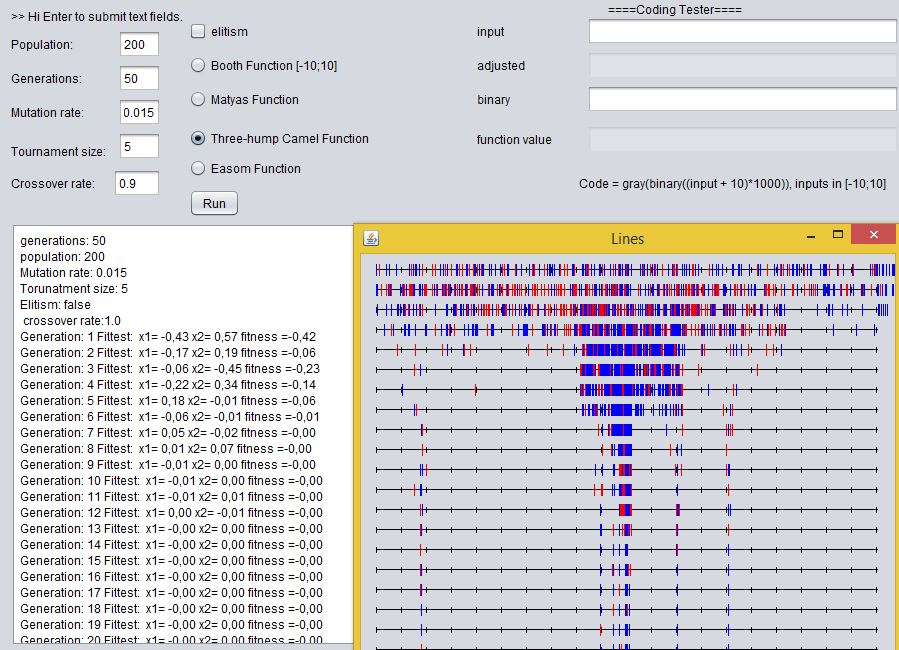
\includegraphics[width=0.7\paperwidth]{genetic}
\caption{Screen of Java genetic function optimiser written by author of this thesis \cite{morph}}
\end{figure}


\subsection{Machine learning}

\section{Conclusions}






All the Web. sources have been checked for availability in November 2015.\\
Web links are not included if articles are to be immediately found with search engines, which is consistent to MLN referencing convention.\\
For modified web documents, date of last modification is shown.


\begin{thebibliography}{9}
 
\bibitem{eggprop} 
Berry D.
\textit{Egg product functional properties} 
American Egg Board Web. 2013

\bibitem{agri} 
Mehdizadeha S., Minaeib S., Hancockc N. H. ,Torshizid M.
\textit{Information Processing in Agriculture}, Volume 1, Issue 2 
Print. 2014

\bibitem{svm} 
Deng X., Wang Q., Chen H., Xie H.
\textit{Eggshell crack detection using a wavelet-based support vector machine} Comput Electron Agric, Print. 2010

\bibitem{nondestr} 
Ketelaerea B.,Bamelisa F., Kempsa1 B., Decuyperea1 E., Baerdemaekera J.
\textit{Non-destructive measurements of the egg quality} World's Poultry Science Journal, Volume 60 / Issue 03,  Cambridge University Press, Print. 2004
 
\bibitem{learnopencv}
Bradski G. ,Kaehler A.
\textit{Learning OpenCV: Computer Vision with the OpenCV Library} O'Reilly Media Inc., Print 2009


\bibitem{performance} 
Gorelick M., Ozsvald I.
\textit{High Performance Python: Practical Performant Programming for Humans} O'Reilly Media Inc., Print 2014

\bibitem{hgtcv} 
Opencv Dev Team
\textit{Hough Circle Transform} OpenCV 2.4.12.0 Documentation, Web. 2014

\bibitem{craters} 
Milbourne A.
\textit{Computers Counting Craters} Birkbeck College, Web. 2012

\bibitem{hgt} 
Rhody, Harvey
\textit{Hough Circle Transform} Chester F. Carlson Center for Imaging Science Rochester Institute of Technology, Web. 2005

\bibitem{mastercv} 
Kapur S., Thakkar N.
\textit{Mastering OpenCV Android Application Programming} Pack Publishing, Print. 2015

\bibitem{fd} 
Opencv Dev Team
\textit{Feature Detection} OpenCV 2.4.12.0 Documentation, Web. 2014

\bibitem{morph} 
Opencv Dev Team
\textit{Morphology Fundamentals: Dilation and Erosion} MathWorks Documentation, The MathWorks, Inc. Web. 2014

\bibitem{erdil} 
Opencv Dev Team
\textit{Eroding and Dilating} OpenCV 2.4.12.0 Documentation, Opencv Dev Team, Web. 2014

\bibitem{cv} 
Shapiro L. G., Stockman G. C
\textit{Computer Vision} Prentice Hall, Print. 2001

\bibitem{cnoisy} 
Khvedchenya E.
\textit{How to detect circles in noisy images} Computer Vision Talks, Web. 2014

\bibitem{featproc} 
Nixon M. S., Aguado A. S.
\textit{Feature Extraction and Image Processing} Academic Press, Print. 2008

\bibitem{gimp} 
Lecarme  O., Delvare K.
\textit{The Book of GIMP: A Complete Guide to Nearly Everything} No Starch Press, Print. 2013

\bibitem{thre} 
Opencv Dev Team
\textit{Image Thresholding.} OpenCV 2.4.12.0 Documentation, Web. 2014

\bibitem{lesscv} 
Barghout L., Sheynin J.
\textit{Real-world scene perception and perceptual organization: Lessons from Computer Vision.} Journal of Vision, Print. 2013

\bibitem{segm} 
Barghout L., Sheynin J.
\textit{Image segmentation} Wikipedia, Wikimedia Foundation Inc, Web. 2015

\bibitem{stackos} 
Gupta V.
\textit{Patchwork Gaurantee spinlocks implicit barrier for PREEMPT\_COUNT} The Linux Kernel Archives, Web. 2013

\bibitem{chibi}
Bate S.
\textit{ChibiOS/RT on the Raspberry Pi} ChibiOS EmbeddedWare Web. 2015

\bibitem{rodos}
Montenegro S., Dannemann F. 
\textit{Real Time Kernel Design for Dependability} DASIA 2009 DAta Systems In Aerospace, Paper. 2009

\bibitem{watershed}
Rosebrock A.
\textit{Watershed OpenCV} PyImageSearch Course, Web. 2015

\end{thebibliography}


\end{document}